\documentclass{standalone}
\usepackage{tikz}

\begin{document}

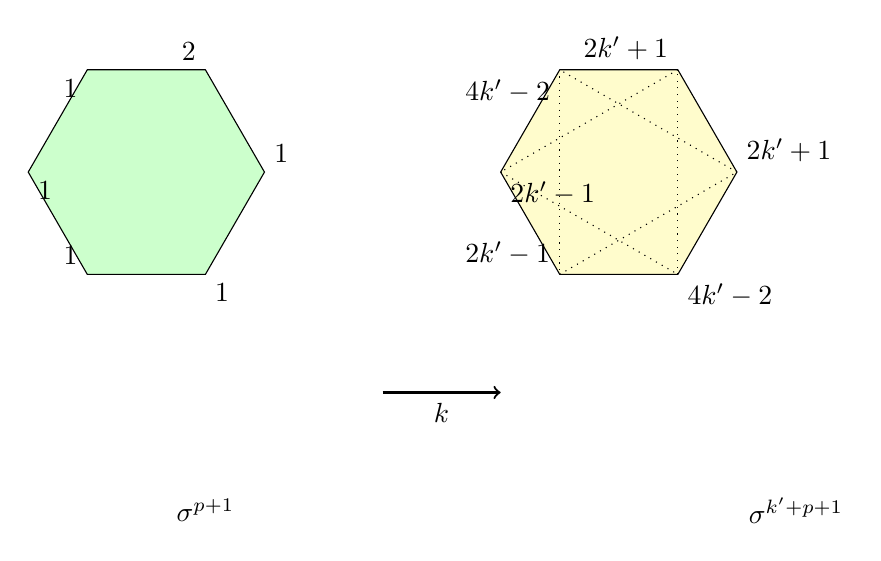
\begin{tikzpicture}[scale=1.5]
    % Define the vertices of the first hexagon
    \coordinate (A) at (0,0);
    \coordinate (B) at (1,0);
    \coordinate (C) at (1.5,0.866);
    \coordinate (D) at (1,1.732);
    \coordinate (E) at (0,1.732);
    \coordinate (F) at (-0.5,0.866);

    % Draw the first hexagon
    \draw[fill=green!20] (A) -- (B) -- (C) -- (D) -- (E) -- (F) -- cycle;

    % Label the vertices of the first hexagon
    \node at (A) [above left] {$1$};
    \node at (B) [below right] {$1$};
    \node at (C) [above right] {$1$};
    \node at (D) [above left] {$2$};
    \node at (E) [below left] {$1$};
    \node at (F) [below right] {$1$};

    % Draw the second hexagon
    \begin{scope}[xshift=4cm]
        \coordinate (A') at (0,0);
        \coordinate (B') at (1,0);
        \coordinate (C') at (1.5,0.866);
        \coordinate (D') at (1,1.732);
        \coordinate (E') at (0,1.732);
        \coordinate (F') at (-0.5,0.866);

        \draw[fill=yellow!20] (A') -- (B') -- (C') -- (D') -- (E') -- (F') -- cycle;
        \draw[dotted] (A') -- (C');
        \draw[dotted] (B') -- (D');
        \draw[dotted] (C') -- (E');
        \draw[dotted] (D') -- (F');
        \draw[dotted] (E') -- (A');
        \draw[dotted] (F') -- (B');

        % Label the vertices of the second hexagon
        \node at (A') [above left] {$2k'-1$};
        \node at (B') [below right] {$4k'-2$};
        \node at (C') [above right] {$2k'+1$};
        \node at (D') [above left] {$2k'+1$};
        \node at (E') [below left] {$4k'-2$};
        \node at (F') [below right] {$2k'-1$};
    \end{scope}

    % Arrow indicating the transformation
    \draw[->, thick] (2.5,-1) -- (3.5,-1) node[midway,below] {$k$};

    % Labels for the transformations
    \node at (1,-2) {$\sigma^{p+1}$};
    \node at (6,-2) {$\sigma^{k'+p+1}$};
\end{tikzpicture}

\end{document}